%form: dc_form_05-07.tex ; user: dc_05-07_purpose_plan_rights.tex
%========== DC =========
%===== p. 05-07 研究の目的・内容、特色、計画、人権 =============
\subsection{研究の目的・内容}
%watermark: w02_purpose_plan_ugly_dc
\newcommand{\研究目的}{%
%begin  研究目的と内容===================

	\setlength\intextsep{0pt}
	\setlength\textfloatsep{0pt}
	\begin{wrapfigure}{r}[7pt]{0.33\linewidth}
		\centering
		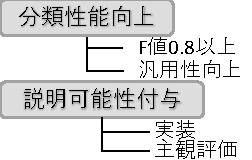
\includegraphics[width=0.33\textwidth]{figs/objects.pdf}
		\vspace{-10mm} 
		\caption{本研究のモデル図}
		\label{fig:objects}
	\end{wrapfigure}

	\vspace{-5mm} 
	\noindent
	●\textbf{研究目的}



	図2の通り、フェイクニュース拡散抑制に向け説明可能な真偽早期検出手法の開発を目指し、
	(1)\textbf{生成コメントを使用した分類でF値が}良好な値とされる\textbf{0.8以上の手法の確立}と、
	(2)\textbf{フェイクニュースの真偽の根拠を説明する手法の確立する手法の確立}を目指す。

	\noindent
	●\textbf{研究方法・研究内容}


	\noindent
	(1) 生成コメントを使用した分類でF値が0.8を上回る手法の確立: 

	早期検出できても誤りが多くユーザから信用が得られぬモデルではなく、
	\textbf{誤りや見逃しなくフェイクニュースを発見するモデル}を構築する。
	%また、性能向上に向く大規模データセットがない場合は条件に符合するものを自作する。
	%最低でもF値0.7以上を目指す。
	また、データセットやモデルの変更で汎用性の向上も目指す。

	\noindent
	(2)フェイクニュースの真偽の根拠を説明する手法の確立:

	SNS上でフェイクニュースの疑いが強い指摘をする場合を想定し、\textbf{生成したコメントを理由付けの題材として活用すること}を目指す。
	また、\textbf{理由付けによるユーザからの信用の変化}を主観実験で評価する。
	コメントを題材とする理由はRTやいいね等と比べ分析しやすい情報を文章として多く提供されるためである。
	%生成コメントから理由付けが難しいならば、実投稿からの実現を目指す。

	\noindent
	●\textbf{所属研究室との関連}

	%所属研究室はエージェント、知的Web、ソフトウェア工学、データマイニングの4つの分野に渡っており、
	%本研究はデータマイニングの一環となる。
	%デマや噂の検出を本研究が扱う対象に含めても
	\textbf{申請者が所属研究室で初めて本研究に着手し、}技術的サポートを除き\textbf{全ての部分を申請者が担当する}。

	\noindent
	●\textbf{研究計画の期間中に異なった研究機関(外国の研究機関等を含む。)において研究に従事することを予定}
	
	申請者は\textbf{期間中1年間タリン工科大学の言語技術研究所(Tanel Alumäe所長)での活動を予定}している。
	このトピックは北米と欧州で研究が盛んで(次項目詳説)、申請者も海外での活動実績が多い(9p.詳説)ため、
	\textbf{最前線の研究に従事する}ためにも申請者が現地で研究に従事することが必要である。

%end  研究目的と内容 ====================
}

\newcommand{\人権の保護及び法令等の遵守への対応}{%
%begin  人権の保護及び法令等の遵守への対応 ===================
	コメント取得を予定してしているSNSはTwitterである。
	Twitter社は2020年3月より学術目的でTwitter APIの利用を自由化しているほか、
	取得したツイートIDを含む情報をデータセットとして公開することも学術目的であれば認められている\cite{twitter_2020}。

	また、先行研究が提供したデータセットを使用する場合は、提供者が示すライセンスやポリシーを遵守する。

	なお、学習済みモデルの公表は平成30年改正著作権法第30条4号により認められている。

	ただし、本研究では主観評価実験としてSNSユーザを対象としたアンケート調査を予定している。
	この調査により収集したデータは、個⼈の特定につながる情報を匿名化した上で解析を⾏い、
	解析結果の公表に際しては、匿名化を⾏ったデータを⽤い、個⼈情報の漏洩防⽌に配慮する。

	{\footnotesize
		\begin{thebibliography}{99}
			\setcounter{enumiv}{11}
			\bibitem{twitter_2020} Twitter開発者ポリシーを分かりやすくアップデート, 2020年3月11日. (最終閲覧日 2020年4月19日) \url{https://blog.twitter.com/developer/ja_jp/topics/tools/2020/DevPolicyUpdate.html}
		\end{thebibliography}
	}
%end  人権の保護及び法令等の遵守への対応 ====================
}

\newcommand{\研究の特色と独創的な点tillNextPage}{%
%begin  研究の特色と独創的な点===================
	\vspace*{-1mm}	
	\noindent
	●\textbf{これまでの先行研究等があれば、それらと比較して、本研究の特色、着眼点、独創的な点}

	%先行研究で既に学術的に実現されている事項と、本研究との差異を記述する。

	ニュースに寄せられそうなコメントを生成する手法は、
	確率分布に従った潜在変数と正解ラベルを使用して頻出単語を生成するTCNN-URGが提案されている\cite{ijcai2018-533}。
	本研究は\textbf{頻出単語を生成するのではなく}、\textbf{説明可能性に繋ぎやすい実際に投稿されたようなコメントを生成する}ことを目指している。

	また、速報性を維持するためにユーザの反応を補完する弱教師あり学習を活用した手法であるMWSSも既に今年提案されている\cite{Shu2020LeveragingMW}。
	コメントに比べ他のユーザの反応(リツイート、いいね、反応したユーザ情報)は説明可能性に繋げにくいため、本研究では生成する対象をコメントに絞っている。

	フェイクニュース自動検出に説明可能性を提供する手法として、
	記事とコメントから真偽判断の決め手となった部分を評価するdEFENDが提案されている\cite{shu2019defend}。
	これは既に投稿されたコメントを対象に含むため、まだコメントが多く寄せられていない状況である\textbf{早期検出を目指す場合には向かない}。
	当研究では、\textbf{生成されたコメントから説明可能性を提供する}ことで早期検出を実現する。
	
	\noindent
	●\textbf{国内外の関連する研究の中での当該研究の位置づけ、意義}

	この研究は、ここ\textbf{数年で社会情勢の変化によって一気に世界的に競争が激化}した一方、
	その\textbf{研究対象が英語に集中}している。
	本研究は早期検出に加え、上記研究の\textbf{知見のローカライズ}も視野に入れている。

	例えば、Google Scholar上で2015年に投稿された中で``fake news''でヒットする論文は\textbf{520本}に対して、
	同じ条件で2019年に投稿された論文は\textbf{15,400本}と実に\textbf{30倍近くに増加}した。
	前項目の通り、この研究分野では頻繁に英語論文が発表されている。
	これに対して、同じ論文プラットフォームで2019年で``フェイクニュース''でヒットする日本語論文は\textbf{169本}と、\textbf{英語の90分の1}にとどまる。
	これは地域による問題意識の差の他にも、近年機械学習やDNNを活用した研究が多いことも考えられる。
	これらの手法に必要な記事と真偽データなどを含む\textbf{大規模データセットが英語に集中している}。
	フェイクニュース検出の場合、ファクトチェック結果をラベル付けに流用することができる\cite{wang-2017-liar}が、
	北米・欧州に比べて日本国内のファクトチェックは発展途上であるため、日本語データセットが少ない。
	もしも日本語を研究対象に含める場合、まずはデータセット作りから着手する必要がある。
	また、同様の理由により\textbf{言語や地域性による差異まで言及した研究はみられない}。
	%具体的には、ユーザへの拡散抑制を呼びかける場合、言語に問わず同じ方法が有効か否か不明である。
	日本国内のユーザに拡散抑制を大きく促すアプローチ方法の検討のためには、この詳細な差異を明らかにすることが必要とみられる。
	%「リフレインさせず飽きさせない」ことと「一貫性をもたせる」ことの両立が難しい……

	\noindent
	●\textbf{本研究が完成したとき予想されるインパクト及び将来の見通し}

	%本研究が完成すると、SNSのユーザへ情報が事実かフェイクかを判断する新しい判断材料を早い段階からもたらすことができる。
	%また、フェイクニュースであることを\textbf{早い段階で説得力がある理由も併せて指摘}することにより、
	%ユーザによる\textbf{拡散を抑制}することができる。
	古今東西で虚偽情報を流布する人々は存在するが、本研究が完成することで\textbf{ユーザが簡単に騙されないような新たな判断材料}を行うことにより、
	\textbf{ジャーナリズムと民主主義に対する最大の脅威であるフェイクニュース}\cite{zhou2019wsdm}から\textbf{ユーザを守る}ことが可能となる。

	さらにフェイクニュース検出にとどまらず、
	前述の言語や国民性に加え、ニュースの分野による生成・分類傾向の差異は\textbf{心理学上においても大きな知見}となり得る。
	更にニュース執筆者に対して\textbf{意図せず誤った情報を発信する前に警告するシステム}など、本研究はあらゆる場面での応用に対応できる。
	
	%\vspace*{-1mm}

	{\footnotesize
		\begin{thebibliography}{99}
			\setcounter{enumiv}{7}
			\vspace*{-2mm}
			\setlength{\parskip}{0cm}
			\setlength{\itemsep}{0cm}
			\begin{spacing}{0.7}
				\bibitem{ijcai2018-533} Feng Qian, \textit{et al.} Neural user response generator: Fake news de-tection with collective user intelligence. In \textit{Proc. of the IJCAI-18}, pp. 3834–3840., 2018.
				\bibitem{Shu2020LeveragingMW} Kai Shu, \textit{et al.} Leveraging multi-source weak social supervision for early detection of fake news. \textit{arXiv}, Vol.abs/2004.01732, 2020.
				\bibitem{wang-2017-liar}William Yang Wang. ``Liar, Liar Pants on Fire'': A New Benchmark Dataset for Fake News Detection. In \textit{Proc. of the 55th Annual Meeting of the Association for Computational Linguistics (Volume 2: Short Papers)}, pp.422-426, 2017.
				\bibitem{zhou2019wsdm}Xinyi Zhou, et al. Fake news: Fundamental theories, detection strategies and challenges. In \textit{Proc. of the WSDM '19}, pp. 836–837, 2019.
			\end{spacing}
		\end{thebibliography}
		%\bibliography{myreferences}
		%\bibliographystyle{junsrt}
	}
%end  研究の特色と独創的な点 ====================
}

\newcommand{\研究計画withVspaceDC}{%
%begin  研究計画 ===================
	% 今年の様式は困ったものです。ブツブツ。
	% 今の技術では「(4)研究計画」のスタート位置を指定できることができません。
	% すみませんが、次の2行を調整してください。
%	\clearpage	% もし「(3) 研究の特色・独創的な点」がp.6に流れこまないなら、この行を有効にしてください。
	\vspace*{12mm}	% 「(4) 研究計画」が正しい高さから始まるように、この値を調整してください。

	%\textbf{この行の高さは、上の「研究の特色・独創的な点」との間隔を\textbackslash vspaceを用いて調整してください。}

	本研究の3年間のスケジュールを以下の図\ref{tbl:chart}に示す。
	申請時点から採用までの期間は、現有のモデルの改善作業によって分類精度の向上を目指すほか、
	以下の計画内のAとBに向くモデルとデータセットの選定や作成の戦術立案を行う。

	%\vspace*{-7mm}
	
	

	\begin{wrapfigure}{r}[7pt]{0.67\textwidth}
		\centering
		\vspace*{-3mm}
		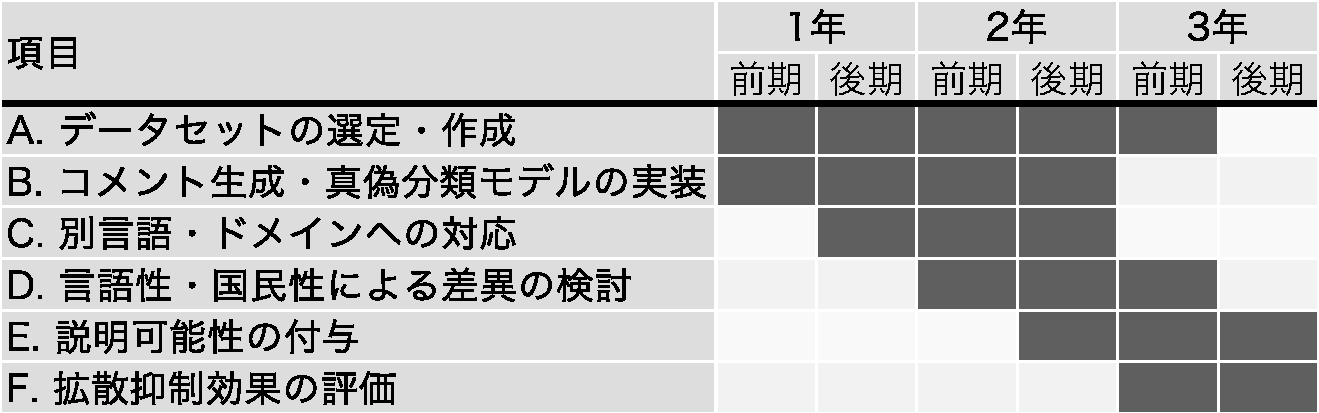
\includegraphics[width=0.67\textwidth]{figs/chart.pdf}
		\vspace*{-10mm}
		\caption{本研究の年次計画(1セルは半期を表す)}
		\label{tbl:chart}
	\end{wrapfigure}
	

	\noindent
	●\textbf{1年目}

	\noindent
	\textbf{A. データセットの選定・作成}

	以下の各タスクで使用するデータセットを随時選定する。
	データセット作成を記述した論文の調査や、Google Dataset Search等の検索エンジンで検索する。
	条件はタスクによるが、少なくともニュースとその真偽、そしてユーザのコメントが必要である。
	もしも条件を満たすデータセットがない場合は、自分で集める必要がある。	

	\noindent
	\textbf{B. コメント生成・真偽分類モデルの実装}

	コメントを生成し分類するモデルの実装を引き続き行う。
	本研究では生成コメントを含めた真偽判定において、分類の総合指標であるF値が0.8を上回ることを目指している。
	もしも現有モデルの拡張では難しい場合は、申請時から着手時までに新たに提案された別手法の調査・拡張を検討している。

	%\noindent
	%\textbf{C. 真偽分類性能向上}

	%本研究では生成コメントを含めた真偽判定において、分類の総合指標であるF値が0.8を上回ることを目指している。
	%データセットの規模拡大やパラメータの調整、分類モデルの変更などで実現を目指す。

	\noindent
	●\textbf{2年目}

	\noindent
	\textbf{C. 別言語・ドメインへの対応}

	言語やニュースのトピックであるドメインの変動に提案モデルを対応させる。
	特に日本語対応する場合、形態素解析や事前学習済み日本語単語の分散表現、そしてデータセットの用意が必要である。
	%また、いずれも同時にデータセットも新たに用意しなければならない。
	もし多言語対応が難しいならば、英語内での別ドメイン対応を予定している。

	\noindent
	\textbf{D. 言語性・国民性による差異の検討}

	Cにより、言語やそれを使用する国民性によってフェイクニュース拡散傾向に違いがみられるか調べる。
	具体的には分類成績や生成されたコメント同士を比較する形で実現する。
	これが国による具体的なフェイクニュースとの触れ方を明らかにし、より具体的な説明可能性の提供や早期検出への道筋となる。

	\noindent
	\textbf{E. 説明可能性の付与}

	ユーザに説明可能性を提供するために、生成されたコメントから真偽を判断した材料を取得する。
	これは生成・分類モデルを拡張することによって実現を目指す。
	また、Dの結果によっては出力の形式を変更・調整するほか、オンライン上でのデモの提供も予定している。
	もしも生成されたコメントから説明可能性が得られない場合は、実際投稿されたコメントと記事から得ることを予定している。

	\noindent
	●\textbf{3年目}

	\noindent
	\textbf{F. 拡散抑制効果の評価}

	実際にSNS上で提供した時を想定し、Bによって分類成績を改善させ、Eによって説明可能性を付与したモデルの効果を測定する。
	具体的には提案モデルがSNSユーザへの拡散意欲やモデルへの信憑性にどのような影響があるか、10点評価によるアンケート調査を用いた主観評価実験で評価する。
	%また、Dに付随しユーザの使用言語によって手法を変えた場合の評価も兼ねる。

%end  研究計画 ====================
}

